\documentclass[a4paper,12pt]{article}
\usepackage[english,ukrainian,russian]{babel}
\linespread{1}
\usepackage{ucs}
\usepackage[utf8]{inputenc}
\usepackage[T2A]{fontenc}
\usepackage[paper=portrait,pagesize]{typearea}
\usepackage{amsmath}
\usepackage{bigints}
\usepackage{amsfonts}
\usepackage{graphicx}
\usepackage{amssymb}
\usepackage{cancel}
\usepackage{gensymb}
\usepackage{multirow}
\usepackage{rotate} 
\usepackage{pdflscape}
\usepackage{bigstrut}
\usepackage[pageanchor]{hyperref}
\usepackage{chngpage}
\usepackage{fancybox,fancyhdr}
\newcommand\tab[1][1cm]{\hspace*{#1}}
\newcommand{\RomanNumeralCaps}[1]{\MakeUppercase{\romannumeral #1}}
\usepackage[left=20mm, top=20mm, right=15mm, bottom=15mm, nofoot]{geometry}


\begin{document}
    \pagestyle{fancy}
    \fancyhead{}
    \fancyhead[R]{ФІ-12 Завалій Олександр}
    \begin{center}
        \large{\textbf{Міністерство освіти і науки України\\
                Національний технічний університет України\\
                «Київський політехнічний інститут імені Ігоря Сікорського»\\
                Навчально-науковий Фізико-технічний інститут}}\\
        \hfill \break \hfill \break \hfill\break \hfill \break \hfill \break \hfill \break \hfill \break
        \hfill \break \hfill \break \hfill \break
        \begin{center}
            \normalsize{\textbf{ОПЕРАЦІЙНІ СИСТЕМИ\\
            Комп’ютерний практикум\\
            Робота №3}}
        \end{center}
    \end{center}
    \hfill \break \hfill \break \hfill \break \hfill \break \hfill \break \hfill \break \hfill \break
    \hfill \break \hfill \break \hfill \break \hfill \break 
    \begin{flushright}
        \large{ \hspace{35pt} Виконав:\\
            студент групи ФI-12\\
            Завалій Олександр\\} 
        \large{ \hspace{35pt} Перевірив:\\
        Кірієнко О.В.} 
    \end{flushright}
    \hfill \break \hfill \break \hfill \break \hfill \break \hfill \break \hfill \break \hfill \break
    \hfill \break
    \begin{center} \textbf{Київ-2023} \end{center}
    \thispagestyle{empty}

\newpage
    \begin{center}
        \section*{\bfseries{Робота №3.\\
        Командна оболонка shell, стандартні
        потоки введення/виведення, фільтри і конвеєри}}
    \end{center}
    \textbf{Мета:} \\
    \hangindent=1.5cm 
    \hangafter=+1 \noindent
    Оволодіння практичними навичками
    перенаправлення стандартних потоків, роботи з
    фільтрами і організації конвеєрів \\
    \begin{center}
        \Large{Варіант №5}
    \end{center}
    Зміст індивідуального завдання:
    \begin{enumerate}
        \item Перейдіть у каталог \textbf{/bin}. Перегляньте список усіх файлів, що починаються із символу \textbf{<<f>>}.
        \item Перегляньте список файлів, імена яких складаються з визначеної у таблиці індивідуальних завдань кількості символів.\textbf{<<2>>}.
        \item Перегляньте список файлів, імена яких починаються із символів \textbf{<<q, r, s, t>>}. Зробіть це декількома способами.
        \item Створіть у вашому домашньому каталозі підкаталог \textbf{lab\_3} і перейдіть в нього.
        \item За допомогою команди \textbf{cat} створіть файл \textbf{my\_text} і запишіть у нього кілька рядків. Потім за допомогою команди \textbf{cat} 
        допишіть у нього ще кілька рядків.
        \item Підрахуйте кількість файлів у каталозі \textbf{/var}, використовуючи і не використовуючи конвеєри. Порівняйте результат.
        \item Підрахуйте кількість файлів у каталозі \textbf{/var}, при цьому зберігши список файлів у файлі \textbf{filelist}, використовуючи команду \textbf{tee}.
        \item Починаючи з вашого домашнього каталогу, виведіть на екран у повному форматі назви усіх файлів і каталогів, що починаються з \textbf{"m"}. 
        При цьому перед виведенням кожної назви на екран повинен виводитися запит на його підтвердження.
        \item Починаючи з кореневого каталогу, виведіть на екран імена всіх каталогів, що останній раз змінювалися більше 15 днів назад.
        \item Виведіть на екран тільки час, що повертається командою \textbf{date}.
        \item Виведіть на екран список усіх користувачів системи, тобто перші поля кожного рядка файлу \textbf{/etc/passwd} (роздільник полів — символ ":").
        \item Виведіть на екран імена усіх файлів у каталозі \textbf{/bin}, що містять слова \textbf{Software} чи \textbf{software}.
         Потік помилок при цьому не повинний виводитися на екран.
        \item Відсортуйте конфігураційний файл вашої оболонки \textbf{(.profile, .cshrc)} відповідно до кодової таблиці ASCII так, щоб при цьому 
        ігнорувалися пробіли на початку рядків. Робіть це з копією файлу, щоби не порушити нормальну працездатність вашої оболонки.
    \end{enumerate}

\newpage
    \begin{center}
        \Large{Task \RomanNumeralCaps{1}}
    \end{center}
    Перейдіть у каталог \textbf{/bin}. Перегляньте список усіх файлів, що починаються із символу \textbf{<<f>>}.
    \begin{figure}[h!]
        \begin{minipage}[h]{1\linewidth}
            \centering
            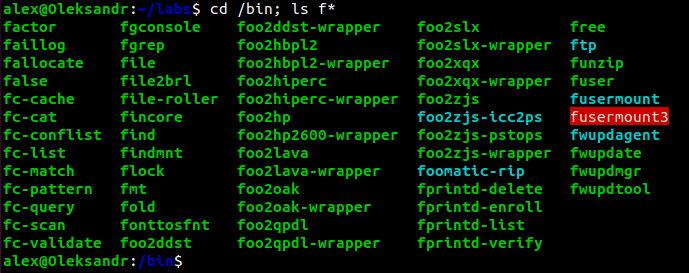
\includegraphics[width=0.6\linewidth]{Prt sc/Figure_1.png}  
        \end{minipage}
    \end{figure}

    \begin{center}
        \Large{Task \RomanNumeralCaps{2}}
    \end{center}
    Перегляньте список файлів, імена яких складаються з визначеної у таблиці індивідуальних завдань кількості символів.\textbf{<<2>>}.
    \begin{figure}[h!]
        \begin{minipage}[h]{1\linewidth}
            \centering
            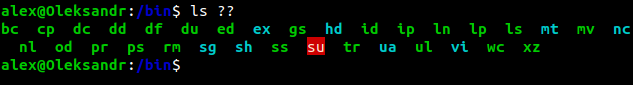
\includegraphics[width=0.5\linewidth]{Prt sc/Figure_2.png}  
        \end{minipage}
    \end{figure}

    \begin{center}
        \Large{Task \RomanNumeralCaps{3}}
    \end{center}
    Перегляньте список файлів, імена яких починаються із символів \textbf{<<q, r, s, t>>}. Зробіть це декількома способами.
    \begin{figure}[h!]
        \begin{minipage}[h]{1\linewidth}
            \centering
            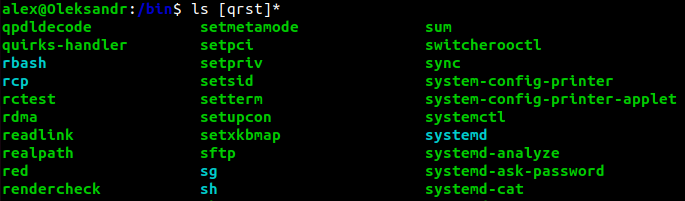
\includegraphics[width=0.5\linewidth]{Prt sc/Figure_3_1.png}  
        \end{minipage}
    \end{figure}
    \begin{figure}[h!]
        \begin{minipage}[h]{1\linewidth}
            \centering
            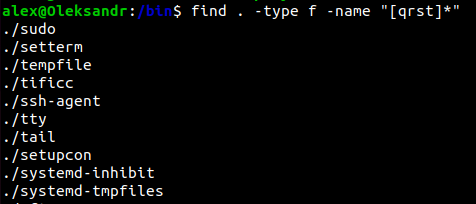
\includegraphics[width=0.5\linewidth]{Prt sc/Figure_3_2.png}  
        \end{minipage}
    \end{figure}

\newpage
    \begin{center}
        \Large{Task \RomanNumeralCaps{4}}
    \end{center}
    Створіть у вашому домашньому каталозі підкаталог \textbf{lab\_3} і перейдіть в нього.
    \begin{figure}[h!]
        \begin{minipage}[h]{1\linewidth}
            \centering
            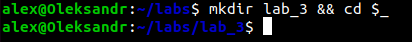
\includegraphics[width=0.5\linewidth]{Prt sc/Figure_4.png}  
        \end{minipage}
    \end{figure}

    \begin{center}
        \Large{Task \RomanNumeralCaps{5}}
    \end{center}
    За допомогою команди \textbf{cat} створіть файл \textbf{my\_text} і запишіть у нього кілька рядків. Потім за допомогою команди \textbf{cat} 
    допишіть у нього ще кілька рядків.
    \begin{figure}[h!]
        \begin{minipage}[h]{1\linewidth}
            \centering
            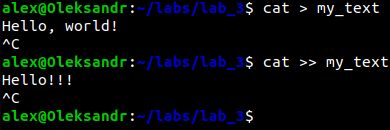
\includegraphics[width=0.5\linewidth]{Prt sc/Figure_5.png}  
        \end{minipage}
    \end{figure}

    \begin{center}
        \Large{Task \RomanNumeralCaps{6}}
    \end{center}
    Підрахуйте кількість файлів у каталозі \textbf{/var}, використовуючи і не використовуючи конвеєри. Порівняйте результат.
    \begin{figure}[h!]
        \begin{minipage}[h]{1\linewidth}
            \centering
            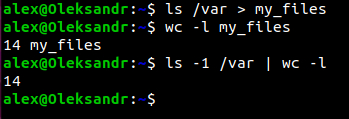
\includegraphics[width=0.5\linewidth]{Prt sc/Figure_6.png}  
        \end{minipage}
    \end{figure}

\newpage
    \begin{center}
        \Large{Task \RomanNumeralCaps{7}}
    \end{center}
    Підрахуйте кількість файлів у каталозі \textbf{/var}, при цьому зберігши список файлів у файлі \textbf{filelist}, використовуючи команду \textbf{tee}.
    \begin{figure}[h!]
        \begin{minipage}[h]{1\linewidth}
            \centering
            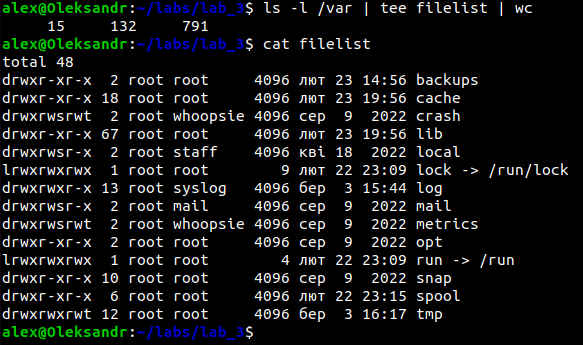
\includegraphics[width=0.5\linewidth]{Prt sc/Figure_7.png}  
        \end{minipage}
    \end{figure}

    \begin{center}
        \Large{Task \RomanNumeralCaps{8}}
    \end{center}
    Починаючи з вашого домашнього каталогу, виведіть на екран у повному форматі назви усіх файлів і каталогів, що починаються з \textbf{"m"}. 
    При цьому перед виведенням кожної назви на екран повинен виводитися запит на його підтвердження.
    \begin{figure}[h!]
        \begin{minipage}[h]{1\linewidth}
            \centering
            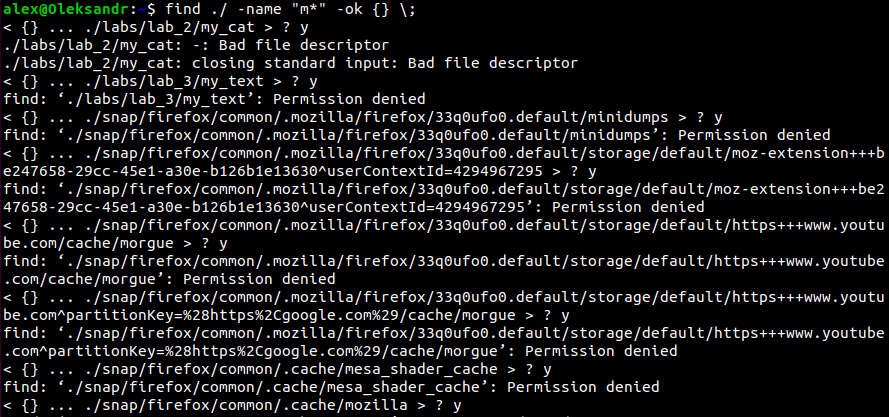
\includegraphics[width=0.8\linewidth]{Prt sc/Figure_8.png}  
        \end{minipage}
    \end{figure}

    \begin{center}
        \Large{Task \RomanNumeralCaps{9}}
    \end{center}
    Починаючи з кореневого каталогу, виведіть на екран імена всіх каталогів, що останній раз змінювалися більше 15 днів назад.
    \begin{figure}[h!]
        \begin{minipage}[h]{1\linewidth}
            \centering
            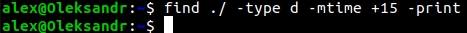
\includegraphics[width=0.5\linewidth]{Prt sc/Figure_9.png}  
        \end{minipage}
    \end{figure} \\

\newpage
    \begin{center}
        \Large{Task \RomanNumeralCaps{10}}
    \end{center}
    Виведіть на екран тільки час, що повертається командою \textbf{date}.
    \begin{figure}[h!]
        \begin{minipage}[h]{1\linewidth}
            \centering
            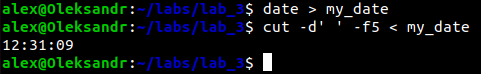
\includegraphics[width=0.5\linewidth]{Prt sc/Figure_10.png}  
        \end{minipage}
    \end{figure}

    \begin{center}
        \Large{Task \RomanNumeralCaps{11}}
    \end{center}
    Виведіть на екран список усіх користувачів системи, тобто перші поля кожного рядка файлу \textbf{/etc/passwd} (роздільник полів — символ ":").
    \begin{figure}[h!]
        \begin{minipage}[h]{1\linewidth}
            \centering
            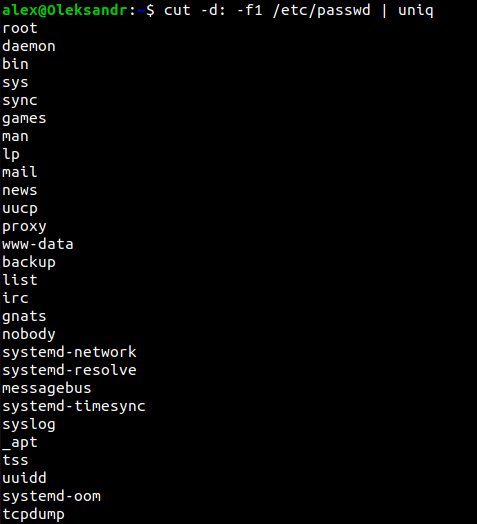
\includegraphics[width=0.5\linewidth]{Prt sc/Figure_11.png}  
        \end{minipage}
    \end{figure}

\newpage
    \begin{center}
        \Large{Task \RomanNumeralCaps{12}}
    \end{center}
    Виведіть на екран імена усіх файлів у каталозі \textbf{/bin}, що містять слова \textbf{Software} чи \textbf{software}.
    Потік помилок при цьому не повинний виводитися на екран.
    \begin{figure}[h!]
        \begin{minipage}[h]{1\linewidth}
            \centering
            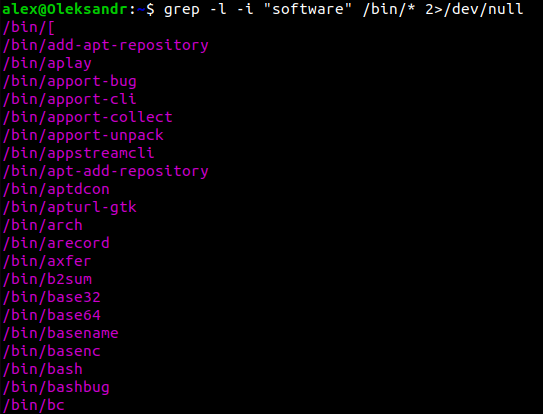
\includegraphics[width=0.5\linewidth]{Prt sc/Figure_12.png}  
        \end{minipage}
    \end{figure}

    \begin{center}
        \Large{Task \RomanNumeralCaps{13}}
    \end{center}
    Відсортуйте конфігураційний файл вашої оболонки \textbf{(.profile, .cshrc)} відповідно до кодової таблиці ASCII так, щоб при цьому 
    ігнорувалися пробіли на початку рядків. Робіть це з копією файлу, щоби не порушити нормальну працездатність вашої оболонки.
    \begin{figure}[h!]
        \begin{minipage}[h]{1\linewidth}
            \centering
            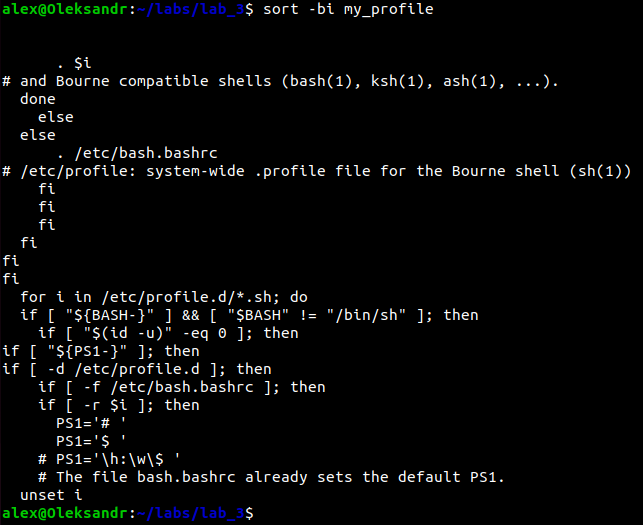
\includegraphics[width=0.7\linewidth]{Prt sc/Figure_13.png}  
        \end{minipage}
    \end{figure}

\newpage
    \begin{center}
        \Large{Висновки}
    \end{center}

    Робота з файлами полягая не тільки в тому, щоб редагувати й переглядати, а ще й у швидкому пошуку інформації, запису 
    результатів виконання та сортуванні інформації.

    Задля забезпечення опрацювання інформаціїй потрібно розміщати її у файлах або відображенні на екрані. Тобто застосувати потоки
    введення/виведення або можливе їх перенаправлення. Тут в нагоді стають метасимволи і правила інтерпретації. Що дає можливість
    зручно демонструвати отримані результати.

    З цього опрацювання випливає подання інформації. Тут в накогоді стає організацію конвеєрів для виконання більш вузьких умов
    згідно завдання. Сюди ж відносяться комани пошуку та команди розділення інформації за ознаками розміщення в певних полях. 
    Також сюди можна додати сортування вхідного потоку, наприклад, за абеткою.

\end{document}